\documentclass[bachelor, och, labwork]{shiza}

\usepackage[utf8]{inputenc}
\usepackage{graphicx}

\usepackage{pdfpages}

\usepackage[sort,compress]{cite}
\usepackage{amsmath}
\usepackage{amssymb}
\usepackage{amsthm}
\usepackage{fancyvrb}
\usepackage{longtable}
\usepackage{array}
\usepackage[english,russian]{babel}
\usepackage{minted}

\usepackage{tempora}


% \usepackage[colorlinks=false]{hyperref}


\newcommand{\eqdef}{\stackrel {\rm def}{=}}


\begin{document}

\title{}

\course{4}

\group{431}

\napravlenie{10.05.01 "--- Компьютерная безопасность}


\author{Никитина Арсения Владимировича}


\satitle{доцент}
\saname{А.\,В.\,Жаркова}


\date{2022}

\maketitle

% Включение нумерации рисунков, формул и таблиц по разделам
% (по умолчанию - нумерация сквозная)
% (допускается оба вида нумерации)
%\secNumbering


\tableofcontents


\section{Задание лабораторной работы}
Стандарт шифрования AES. Перемножить байты:
\begin{center}
    $(1,1,0,1,0,0,1,1) \cdot (0,1,1,1,0,0,1,1)$,

    $(0,1,0,1,0,1,0,1) \cdot (1,0,1,0,1,0,1,0)$
\end{center}


\section{Теоретическая часть}

Алгоритм AES оперирует с байтами, которые интерпретируются как элементы 
поля $GF(2^8)$. В данном поле определены операции сложения и умножения двух элементов,
причем результатом такого умножения будет точно элемент данного поля.

Итак, для того, чтобы выполнить умножение двух байтов $p$ и $q$, каждый из байтов 
требуется представить в виде полинома:

\begin{center}

$p(x) = p_7x^7+p_6x^6+p_5x^5+p_4x^4+p_3x^3+p_2x^2+p_1x+p_0, ~p_i \in$ \{0,1\};

$q(x) = q_7x^7+q_6x^6+q_5x^5+q_4x^4+q_3x^3+q_2x^2+q_1x+q_0, ~q_i \in$ \{0,1\}.
\end{center}

Умножение байт в таком представлении производится по модулю неприводимого в $GF(2^8)$
многочлена $f(x)=x^8+x^4+x^3+x+1$, то есть получаем конечную формулу:

\begin{center}
    $r(x) \equiv p(x)q(x) ~(mod ~f(x))$
\end{center}

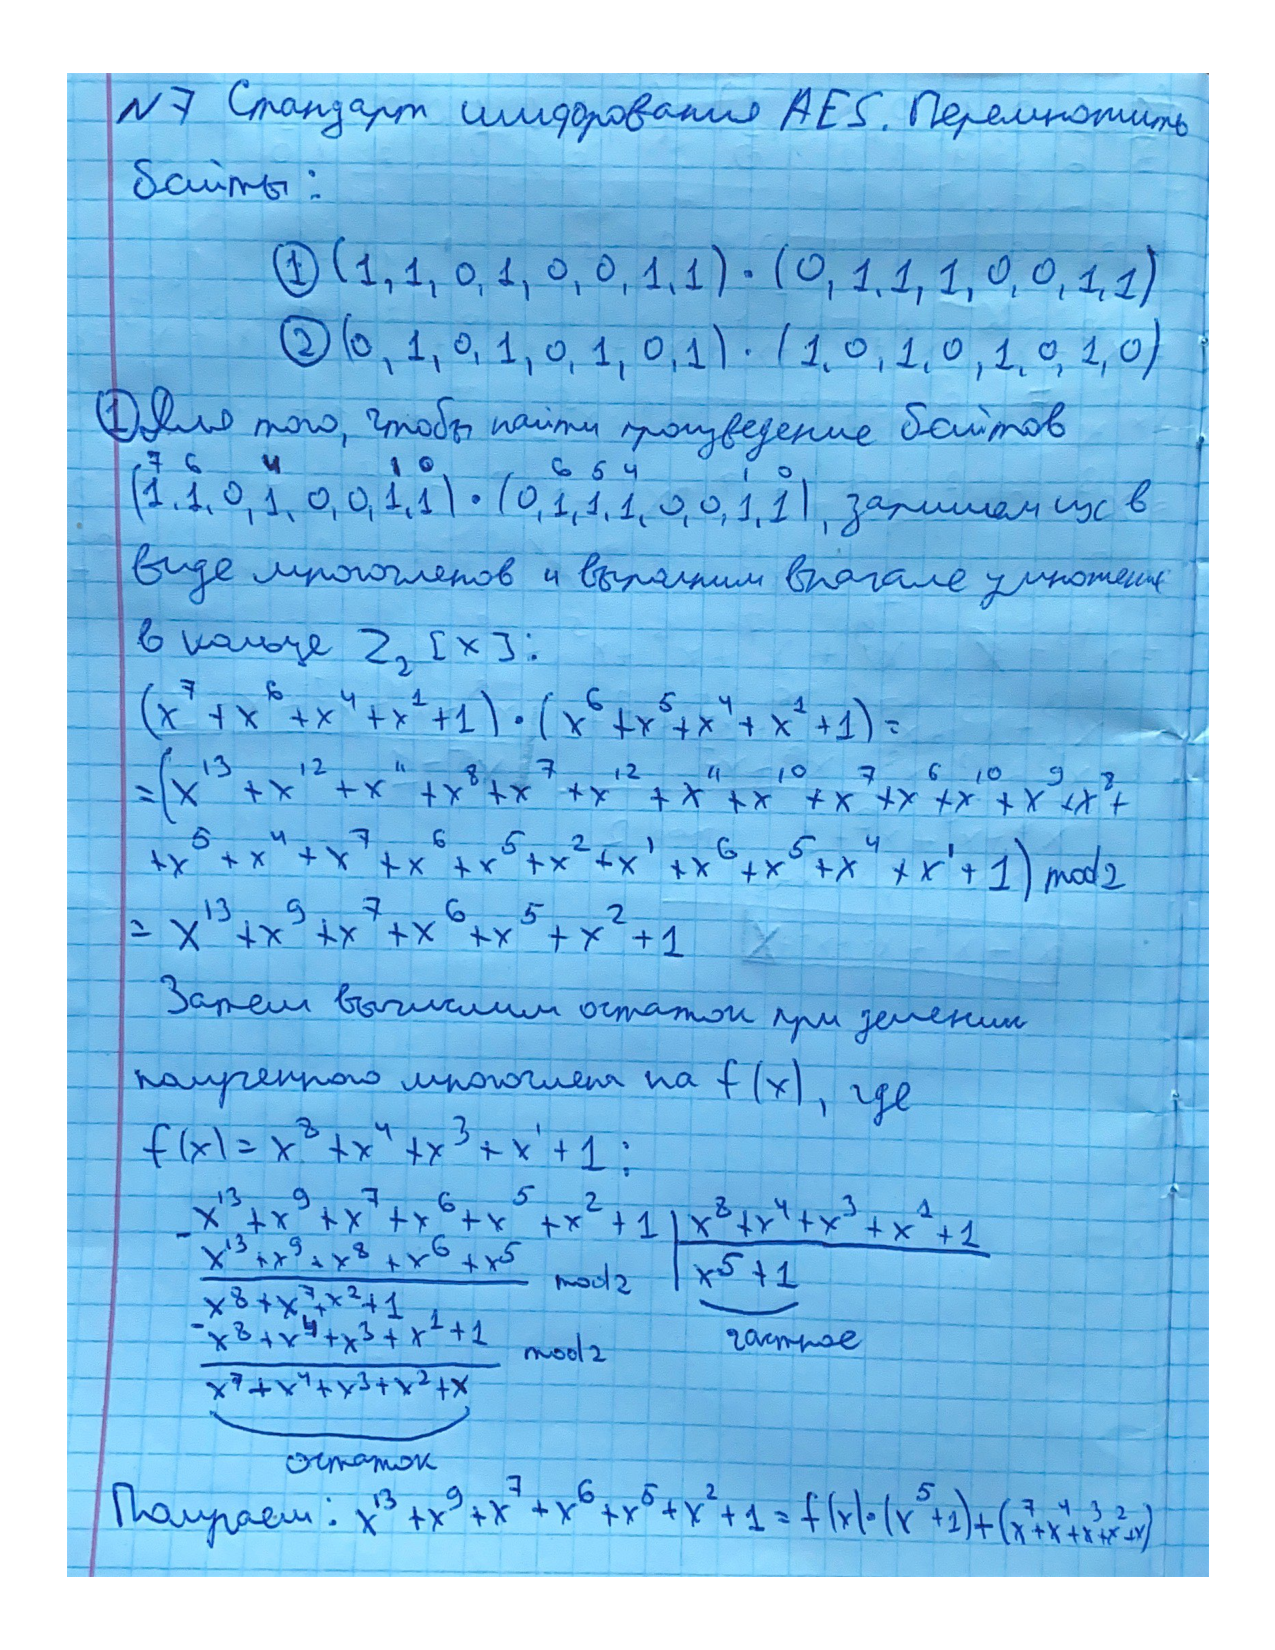
\includepdf[pages={1}, pagecommand=\section{Практическая часть}]{7.pdf}
\includepdf[pages={2}]{7.pdf}\nopagebreak

\end{document}